\section[toc=Quasi-elastic scattering]{Quasi-elastic scattering \\ \small{Building a generator step by step}}

\begin{wideslide}[toc=QEL on free N]{Quasi-elastic scattering on a free nucleon}
\null\vfill

  \myBox{Llewellyn-Smith formula}
  
  $$\frac{d\sigma}{d|q^2|} {{\nu_l + n \rightarrow l^- + p}\choose{\bar\nu_l + p \rightarrow l^+ + n}} = \frac{M^2G_F^2\cos\theta_C}{8\pi E_\nu^2}\left[A(q^2) \mp B(q^2)\frac{(s - u)}{M^2} + C(q^2)\frac{(s - u)^2}{M^4}\right]$$
  
  \myBox{Notation}
  
  \begin{itemize}
    \item Constants: $M$ - nucleon mass, $G_F$ - Fermi constant, $\theta_C$ - Cabibbo angle,
    \item $q^2 = (k - k')^2 = (p' - p)^2$ - four-momentum squared, where $k$, $k'$, $p$, $p'$ are four-momenta of initial and final lepton, initial and final nucleon
    \item $E_\nu$ - neutrino energy
    \item $s = (k + k')^2$ and $u = (k - p')^2$ - Mandelstam variables
  \end{itemize}

  
\vfill\null
\end{wideslide}

\begin{wideslide}[toc=]{Quasi-elastic scattering on a free nucleon}
\null\vfill

  \myBox{Llewellyn-Smith formula}
  
  $$\frac{d\sigma}{d|q^2|} {{\nu_l + n \rightarrow l^- + p}\choose{\bar\nu_l + p \rightarrow l^+ + n}} = \frac{M^2G_F^2\cos\theta_C}{8\pi E_\nu^2}\left[A(q^2) \mp B(q^2)\frac{(s - u)}{M^2} + C(q^2)\frac{(s - u)^2}{M^4}\right]$$
  
  \myBox{General idea}
  
  \begin{itemize}
    \item Having $k$ and $p$, generate $k'$ and $p'$
    \item Calculate $q^2$ and $(s - u) = 4ME_\nu + q^2 -m^2$ based on generated kinematics
    \item Calculate cross section
    \item Repeat $N$ times and the result is given by: 
    
    $$\sigma_{total} \sim \frac{1}{N} \sum\limits_{i = 1}^N \sigma (q_i^2)$$
    
  \end{itemize}

\vfill\null
\end{wideslide}

\begin{slide}{Generating kinematics}
\null\vfill

  \twocolumn
{
\centering
\begin{tikzpicture}

  \draw [notFilled=pdcolor3, thin] (-0.5, -0.5) -- (-0.5, 1.5) -- node[below, yshift = -0.25 cm] {\color{pdcolor1}LAB} (3.5, 1.5) -- (3.5, -0.5) -- (-0.5, -0.5);

  \draw [filled = pdcolor1] (0, 0) circle (0.25);
  \draw [filled = pdcolor6] (3, 0) circle (0.25);
  \draw [line, ultra thick, ->] (0.25, 0) -- node[above] {$\vec p_\nu$} (1.5, 0);
  \draw [line, ultra thick, ->, color = pdcolor6] (2.75, 0.1) -- node[above, xshift = 0.25cm] {$\vec p_N$} (2.0, 0.5);

\end{tikzpicture}
}
{
\centering
\begin{tikzpicture}

  \draw [notFilled=pdcolor3, thin] (-0.5, -0.5) -- (-0.5, 1.5) -- node[below, yshift = -0.25 cm] {\color{pdcolor1}CMS} (3.5, 1.5) -- (3.5, -0.5) -- (-0.5, -0.5);

  \draw [filled = pdcolor1] (0, 0) circle (0.25);
  \draw [filled = pdcolor6] (3, 0) circle (0.25);
  \draw [line, ultra thick, ->] (0.25, 0) -- node[above] {$\vec p*$} (1.25, 0);
  \draw [line, ultra thick, ->, color = pdcolor6] (2.75, 0) -- node[above] {$\vec p*$} (1.75, 0);

\end{tikzpicture}
}

  \begin{itemize}
    \item Lets consider kinematics in center-of-mass system
    \item Mandelstam $s$ is invariant under Lorentz transformation
   
    $$s = (k + p)^2 = (E + E_p)^2 - (\vec k + \vec p)^2 = (E^* + E_p^*)^2$$
   
    \item $\sqrt{s}$ is the total energy in CMS

    $$\sqrt{s} = E^* + E_p^* = \sqrt{p^{*2} + m^2} + \sqrt{p^{*^2} + M^2}$$
    
    \item We will use it to calculate $p*$
   
  \end{itemize}

\vfill\null
\end{slide}

\begin{slide}[toc=]{Generating kinematics}
\null\vfill
  
  \begin{itemize}
   \item Lets do some simple algebra:

  \vspace{-10pt}
  \begin{eqnarray*}
    \sqrt{s} & = & E^* + E_p^* = \sqrt{p^{*2} + m^2} + \sqrt{p^{*^2} + M^2} \\
    \sqrt{s} & = & E^* + \sqrt{E^{*2} - m^2 + M^2} \\
    s & = & E^{*2} + E^{*2} - m^2 + M^2 + 2E^*E_p^* \\
    s & = & 2E^*(E^* + E_p^*) - m^2 + M^2 \\
    s & = & 2E^*\sqrt{s} - m^2 + M^2 \\
    E^* & = & \frac{s + m^2 - M^2}{2\sqrt{s}} \\
    E_p^* & =&  \frac{s + M^2 - m^2}{2\sqrt{s}} \mbox{ (analogously)}
  \end{eqnarray*}
  
  \item After more algebra we get:
  
  \vspace{-10pt}
  $$p^* = \sqrt{E^{*2} - m^2} = \frac{[s - (m - M)^2]\cdot[s - (m + M)^2]}{2\sqrt{s}}$$

  \end{itemize}

\vfill\null
\end{slide}

\begin{slide}[toc=]{Generating kinematics}
\null\vfill

  \twocolumn
  {
    \sep
    \begin{itemize}
      \item We use spherical coordinate system to determine momentum direction in CMS:
    \end{itemize}
    $$\vec p^* = p^* \cdot (\sin\theta\cos\phi,~~\sin\theta\sin\phi,~~\cos\theta)$$
  }
  {
    \centering\tdplotsetmaincoords{60}{110}

\pgfmathsetmacro{\rvec}{.8}
\pgfmathsetmacro{\thetavec}{45}
\pgfmathsetmacro{\phivec}{60}

\begin{tikzpicture}[scale = 2, tdplot_main_coords]

  \coordinate (O) at (0,0,0);
  \draw[thick, >=latex, ->] (0,0,0) -- (1,0,0) node[anchor=north east]{$x$};
  \draw[thick, >=latex, ->] (0,0,0) -- (0,1,0) node[anchor=north west]{$y$};
  \draw[thick, >=latex, ->] (0,0,0) -- (0,0,1) node[anchor=south]{$z$};
  
  \tdplotsetcoord{P}{\rvec}{\thetavec}{\phivec}
  
  \draw[-stealth, color = pdcolor6] (O) -- (P) node[above right] {$p^*$};
  \draw[dashed, color = pdcolor6] (O) -- (Pxy);
  \draw[dashed, color = pdcolor6] (P) -- (Pxy);

  \tdplotdrawarc[color = pdcolor3]{(O)}{0.2}{0}{\phivec}{anchor=north}{$\phi$}

  \tdplotsetthetaplanecoords{\phivec}
  
  \tdplotdrawarc[tdplot_rotated_coords, color = pdcolor3]{(0,0,0)}{0.5}{0}{\thetavec}{anchor=south west}{$\theta$}

\end{tikzpicture}
  }  

  \begin{itemize}
    \item Generate random angles:  
    \item[]
    
    \begin{tabular}{rclll}
           $\phi$ & $ = $ &  $2\pi\cdot\mbox{random}[0,1]$ & $\Rightarrow$ & $\sin\phi,~~\cos\phi$ \\ \\
     $\cos\theta$ & $ = $ & $2\cdot\mbox{random}[0,1] - 1$ & $\Rightarrow$ & $\sin\theta, ~~\cos\theta$  
    \end{tabular}
    
    \item[]
    
    \item All we need to do is to go back to LAB frame

  \end{itemize}

\vfill\null
\end{slide}

\begin{slide}{LAB $\leftrightarrows$ CMS}
\null\vfill

  \begin{itemize}
    
    \item Lorentz boost in direction $\hat n = \frac{\vec v}{v}$ of $(t,\vec r)$:
    
    \begin{eqnarray*}
      t' & = & \gamma \left(t - v \hat n\cdot\vec r\right) \\
      \vec r' & = & \vec r + (\gamma - 1)(\hat n\cdot\vec r)\hat n - \gamma t v \hat n
    \end{eqnarray*}
    
  \end{itemize}
  
  \sep
  
  \twocolumn
  {
    \begin{itemize}
      
      \item In our case
  
      $$\vec v = \frac{\vec p_\nu + \vec p_N}{E_\nu + E_N}$$
    
      \item Boost from LAB to CMS in $\vec v$ direction
    
      \item Boost from CMS to LAB in $-\vec v$ direction
    
    \end{itemize}
  }
  {
    \begin{tikzpicture}

  \draw [notFilled=pdcolor3, thin] (-0.5, -0.5) -- (-0.5, 1.5) -- node[below, yshift = -0.25 cm] {\color{pdcolor1}LAB} (3.5, 1.5) -- (3.5, -0.5) -- (-0.5, -0.5);

  \draw [filled = pdcolor1] (0, 0) circle (0.25);
  \draw [filled = pdcolor6] (3, 0) circle (0.25);
  \draw [line, ultra thick, ->] (0.25, 0) -- node[above] {$\vec p_\nu$} (1.5, 0);
  \draw [line, ultra thick, ->, color = pdcolor6] (2.75, 0.1) -- node[above, xshift = 0.25cm] {$\vec p_N$} (2.0, 0.5);

\end{tikzpicture}

\sep

\begin{tikzpicture}

  \draw [notFilled=pdcolor3, thin] (-0.5, -0.5) -- (-0.5, 1.5) -- node[below, yshift = -0.25 cm] {\color{pdcolor1}CMS} (3.5, 1.5) -- (3.5, -0.5) -- (-0.5, -0.5);

  \draw [filled = pdcolor1] (0, 0) circle (0.25);
  \draw [filled = pdcolor6] (3, 0) circle (0.25);
  \draw [line, ultra thick, ->] (0.25, 0) -- node[above] {$\vec p*$} (1.25, 0);
  \draw [line, ultra thick, ->, color = pdcolor6] (2.75, 0) -- node[above] {$\vec p*$} (1.75, 0);

\end{tikzpicture}

  }
  
\vfill\null
\end{slide}

\begin{wideslide}[toc=Cross section]{Calculating cross section}
\null\vfill

  \myBox{Llewellyn-Smith formula}
  
  $$\frac{d\sigma}{d|q^2|} {{\nu_l + n \rightarrow l^- + p}\choose{\bar\nu_l + p \rightarrow l^+ + n}} = \frac{M^2G_F^2\cos\theta_C}{8\pi E_\nu^2}\left[A(q^2) \mp B(q^2)\frac{(s - u)}{M^2} + C(q^2)\frac{(s - u)^2}{M^4}\right]$$
  
  \myBox{Calculation}

  \begin{itemize}
    \item Once we have $p'$ and $k'$ in LAB frame we can calculate $q^2$ and $(s - u)$
    \item Once we have $q^2$ we can calculate $A(q^2)$, $B(q^2)$, $C(q^2)$
    \item We have everything to calculate cross section
    \item Do we? Or maybe we are still missing something?
  \end{itemize}

\vfill\null
\end{wideslide}

\begin{wideslide}[toc=]{Calculating cross section}
\null\vfill

  \myBox{Llewellyn-Smith formula}
  
  $$\frac{d\sigma}{d|q^2|} {{\nu_l + n \rightarrow l^- + p}\choose{\bar\nu_l + p \rightarrow l^+ + n}} = \frac{M^2G_F^2\cos\theta_C}{8\pi E_\nu^2}\left[A(q^2) \mp B(q^2)\frac{(s - u)}{M^2} + C(q^2)\frac{(s - u)^2}{M^4}\right]$$
  
  \myBox{Calculation}

  \begin{itemize}
    \item Once we have $p'$ and $k'$ in LAB frame we can calculate $q^2$ and $(s - u)$
    \item Once we have $q^2$ we can calculate $A(q^2)$, $B(q^2)$, $C(q^2)$
    \item We have everything to calculate cross section
    \item Do we? Or maybe we are still missing something?
  \end{itemize}
  \sep
  \centering{\color{pdcolor6} We change the variable we integrate over! We need Jacobian!}

\vfill\null
\end{wideslide}

\begin{wideslide}[toc=]{Calculating cross section}
\null\vfill

  \begin{itemize}
    
    \item Express $q^2$ in terms of angle:
    
    $$q^2 = (k - k')^2 = m^2 - 2kk' = m^2 - 2EE' + 2|\vec k||\vec k'|\cos\theta $$
    
    \item Thus, the Jacobian is given by:
    
    $$dq^2 = 2|\vec k||\vec k'|d(\cos\theta)$$
    
    {\it\color{pdcolor3}Note: must be calculated in CMS}
    
    \item Total cross section is given by:
    
    {\small
    \begin{eqnarray*}
      \sigma      & = & \int\limits_{-1}^{1} \frac{M^2G_F^2\cos\theta_C}{8\pi E_\nu^2}\left[A(q^2) \mp B(q^2)\frac{(s - u)}{M^2} + C(q^2)\frac{(s - u)^2}{M^4}\right]2|\vec k||\vec k'|d\cos\theta \\
      \sigma_{MC} & = & \frac{2}{N}\sum\limits_{i = 1}^N \frac{M^2G_F^2\cos\theta_C}{8\pi E_\nu^2}\left[A(q_i^2) \mp B(q_i^2)\frac{(s_i - u_i)}{M^2} + C(q_i^2)\frac{(s_i - u_i)^2}{M^4}\right]2|\vec k_i||\vec k'_i|
    \end{eqnarray*}
    }
  \end{itemize}

\vfill\null
\end{wideslide}

\begin{slide}[toc=]{Calculating cross section}
\null\vfill

  \twocolumn
  {
    \sep
    \begin{itemize}
      \item We want to avoid any sharp peaks
      \item They affect our efficiency and accuracy
      \item Lets change variable once again:
      
      $$\cos\theta = 1 - 2x^2$$
     
      where $x\in[0,1]$
      
      \item Note extra Jacobian and new integration limits
      
    \end{itemize}
    
    \vspace{-20pt}$$\hspace*{-20pt}2\int\limits_{-1}^1 d(\cos\theta) \rightarrow \int\limits_1^0 dx (-4x) \rightarrow \int\limits_0^1 4xdx$$
  }
  {
    \usetikzlibrary{calc}

\pgfplotsset{every  tick/.style={pdcolor3,}, minor x tick num=1,}

\begin{tikzpicture}

  \begin{axis}[xlabel = {$\cos\theta$}, ylabel = {$\frac{d\sigma}{d\cos\theta}$ [arbitrary units]}, ylabel near ticks, domain=-1:1, scale=0.5, axis lines = left, inner axis line style={>=latex}, ymin = 0, ymax = 1.2, xmin = -1, xmax = 1.2]
    
    \addplot [thick, color = pdcolor6] table[x = x, y = y, col sep = space, mark = none] {data/qelKinCos.dat};
    
  \end{axis}

\end{tikzpicture}
    \vspace{-10pt}
    \usetikzlibrary{calc}

\pgfplotsset{every  tick/.style={pdcolor3,}, minor x tick num=1,}

\begin{tikzpicture}

  \begin{axis}[xlabel = {$x$}, ylabel = {$\frac{d\sigma}{dx}$ [arbitrary units]}, ylabel near ticks, domain=0:1, scale=0.5, axis lines = left, inner axis line style={>=latex}, ymin = 0, ymax = 1.2, xmin = 0, xmax = 1.2]
    
    \addplot [thick, color = pdcolor6] table[x = x, y = y, col sep = space, mark = none] {data/qelKinX.dat};
    
  \end{axis}

\end{tikzpicture}
  }
  
\vfill\null
\end{slide}

\begin{wideslide}[toc=]{Calculating cross section}
\null\vfill

  \begin{itemize}
    
    \item Finally, the cross section is given by:
    
    {\small
    \begin{eqnarray*}
      \sigma      & = & \int\limits_{0}^{1} \frac{M^2G_F^2\cos\theta_C}{8\pi E_\nu^2}\left[A(q^2) \mp B(q^2)\frac{(s - u)}{M^2} + C(q^2)\frac{(s - u)^2}{M^4}\right]2|\vec k||\vec k'|4xdx \\
      \sigma_{MC} & = & \frac{1}{N}\sum\limits_{i = 1}^N \frac{M^2G_F^2\cos\theta_C}{8\pi E_\nu^2}\left[A(q_i^2) \mp B(q_i^2)\frac{(s_i - u_i)}{M^2} + C(q_i^2)\frac{(s_i - u_i)^2}{M^4}\right]2|\vec k_i||\vec k'_i|4x
    \end{eqnarray*}
    }
    
    \item In conclusion: do some kinematics and some boosts between CMS and LAB, change integration variable several times... and you are ready to calculate total cross section
    
    \item Now we need to generate some events. We want them to be distributed according to our cross section formula.
      
  \end{itemize}

\vfill\null
\end{wideslide}

\begin{slide}{Generating events}
\null\vfill

  \twocolumn
  {
    \begin{itemize}
      \item Generate $x \in [0:1]$
      \item Do kinematics
    \end{itemize}
      \begin{eqnarray*}
	x & \rightarrow & \cos\theta \\
	\cos\theta & \rightarrow & k'^*, p'^* \\
	k'^*, p'^* & \rightarrow & k', p' \\
	& \vdots &
      \end{eqnarray*}
    \begin{itemize}
      \item Calculate cross section $\sigma$
    \end{itemize}
  }
  {
    \sep\sep\sep
    \usetikzlibrary{calc}

\pgfplotsset{every  tick/.style={pdcolor3,}, minor x tick num=1,}

\begin{tikzpicture}

  \begin{axis}[xlabel = {$x$}, ylabel = {$\frac{d\sigma}{dx}$ [arbitrary units]}, ytickmax = 0.0, ylabel near ticks, domain=0:1, scale=0.5, axis lines = left, inner axis line style={>=latex}, ymin = 0, ymax = 1.2, xmin = 0, xmax = 1.2]
    
    \addplot [thick, color = pdcolor6] table[x = x, y = y, col sep = space, mark = none] {data/qelKinX.dat};
    \addplot [thin, color = pdcolor3, dashed] coordinates {(0, 1) (0.8, 1)};
    
    \node[right] at (axis cs: 0.8, 1.0) {$\sigma_{max}$};
    
  \end{axis}

\end{tikzpicture}
  }
  
  \begin{itemize}
  
    \item Accept an event with the probability given by
    
    $$P = \frac{\sigma}{\sigma_{max}}$$
    \vspace{-15pt}
    \item And you almost have you MC neutrino-event generator, just a few more steps...
  \end{itemize}

\vfill\null
\end{slide}

\begin{slide}{A few more steps}
\null\vfill

  \begin{itemize}
    \item add other dynamics: resonance pion production, deep inelastic scattering...
    \item add support for nucleus as a target 
    \item if you have nucleus add some two-body current interactions
    \item if you have nucleus add some nuclear effects: Pauli blocking, final state interactions, formation zone...
  \end{itemize}
  
  \twocolumn
  {
    \begin{itemize}
      \item add support for neutrino beam
      \item add support for detector geometry
      \item add some interface to set up simulations parameters and saving the output
      \item and your MC is done!
    \end{itemize}
  }
  {
    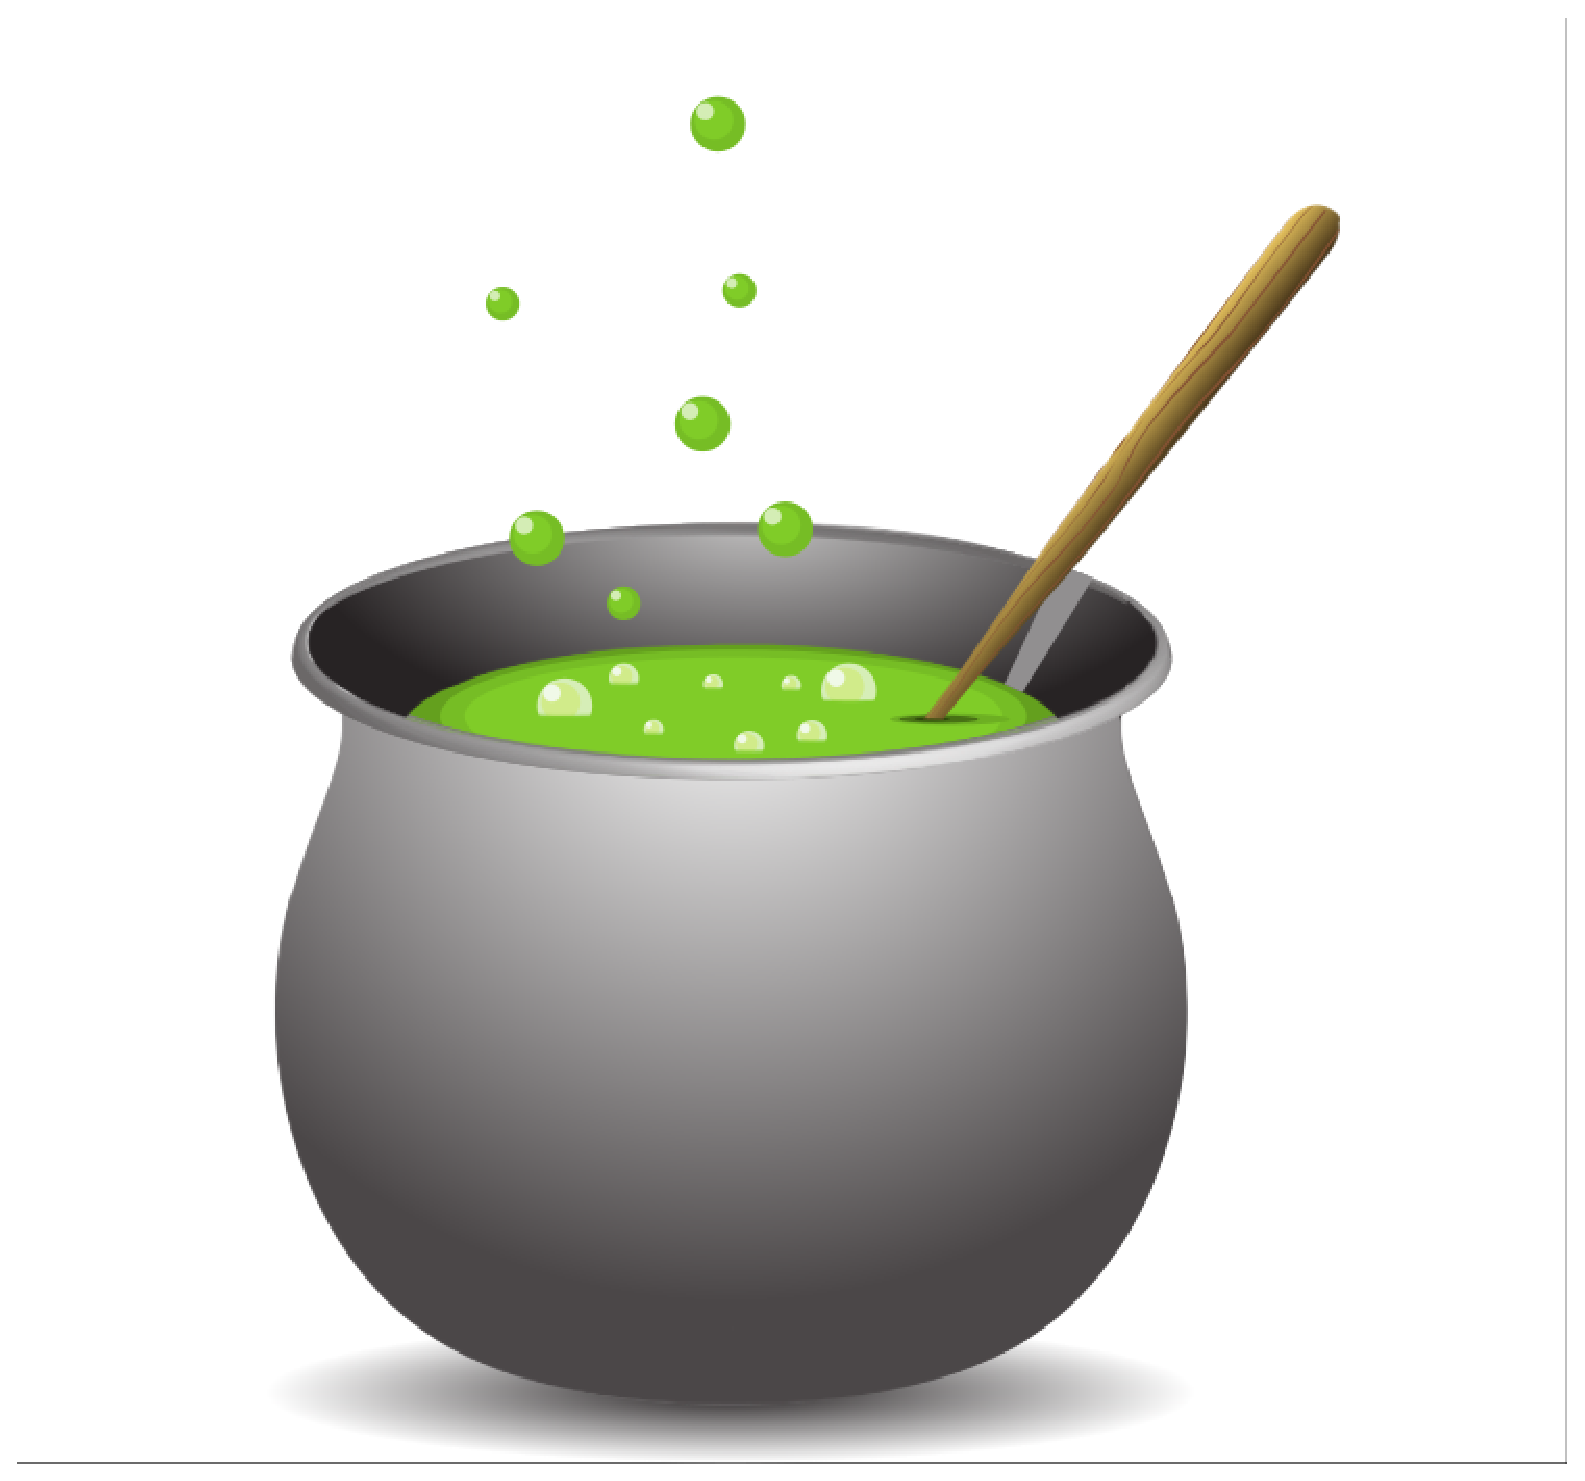
\includegraphics[width=\columnwidth]{figures/kociol.eps}
  }

\vfill\null
\end{slide}